\documentclass[a4paper,11pt]{report}
\usepackage[french]{babel}
\usepackage[T1]{fontenc}
\usepackage[utf8]{inputenc}
\usepackage{lmodern}
\usepackage{microtype}
\usepackage{hyperref}
\usepackage{tabulary}
\usepackage{framed}
\usepackage{fancyhdr}
\usepackage{amsmath}
\usepackage{bbm}
\usepackage{graphicx}
%\usepackage{pst-all}
%\usepackage{xcolor}
%\usepackage{nopageno}

%\newcommand{\latin}[1]{\textit{#1}}

\usepackage[margin=1.0in]{geometry}

%%%%%%%%%%%%%%
%\usepackage{geometry}
 %\geometry{
% a4paper,
 %total={210mm,297mm},
 %left=20mm,
 %right=20mm,
 %top=20mm,
 %bottom=20mm,
 %}
 %%%%%%%%%%%%%%
 
\pagestyle{empty}

\pagestyle{fancy}
\fancyhead{}
\renewcommand{\headrulewidth}{0.5pt}
\fancyhead[R]{\textit{\nouppercase{\rightmark}}}
\fancyfoot{}
\renewcommand{\footrulewidth}{0.5pt}
\fancyfoot[L]{\textit{\nouppercase{\leftmark}}}
\fancyfoot[R]{\thepage}
  
\begin{document}
	\begin{titlepage}
		\vspace*{\stretch{2}}
		\begin{center}
			\large\bfseries\itshape Stage ETE 2015\\
		\end{center}
		\noindent\rule{\linewidth}{3pt}

		\begin{center}
			\Huge\bfseries\itshape Description du système\\
		\end{center}
		
		\noindent\rule{\linewidth}{3pt}
		\begin{center}
			\bfseries
			\large F-PHT \\
			\large Un système d'index de filtres de Bloom pour la recherche d'information par mots clés
		\end{center}
		\vspace*{\stretch{2}}
		\begin{center}
			Réalisé par \textbf{DOAN} Cao Sang \\
			Encadrant: M. \textbf{MAKPANGOU} Mesaac, Regal
		\end{center}
		\vspace*{\stretch{0.5}}
		\begin{center}
			1 Juillet 2015
		\end{center}
	\end{titlepage}

\tableofcontents

\chapter{Vue globale}
\section{Prefix Hash Tree (PHT)}
	Un arbre préfixe est un arbre numérique ordonné qui est utilisé pour stocker une table associative où les clés sont généralement des chaînes de caractères. Contrairement à un arbre binaire de recherche, aucun nœud dans le trie ne stocke la chaîne à laquelle il est associé. C'est la position du nœud dans l'arbre qui détermine la chaîne correspondante\footnote{Wikipédia}.
	
	Pour tout nœud, ses descendants ont en commun le même préfixe. La racine est associée à la chaîne vide. Des valeurs ne sont pas attribuées à chaque nœud, mais uniquement aux feuilles et à certains nœuds internes se trouvant à une position qui désigne l'intégralité d'une chaîne correspondante à une clé.
	
	Pour faire une recherche d'une valeur associée à une clé, au départ, on se situe à la racine de l'arbre, en prenant le premier élément de la clé de la requête, on trouve le chemin étiqueté par cet élément, s'il n'existe pas, on est sûr que cette clé n'est pas dans l'arbre. Dès que l'on trouve le chemin, on arrive sur le bon nœud et continue en prenant le deuxième élément de la clé de requête, on applique cette méthode jusqu'à quand on trouve cette clé et se termine sur une feuille.
	
	\begin{figure}[!htbp]
	\centering
	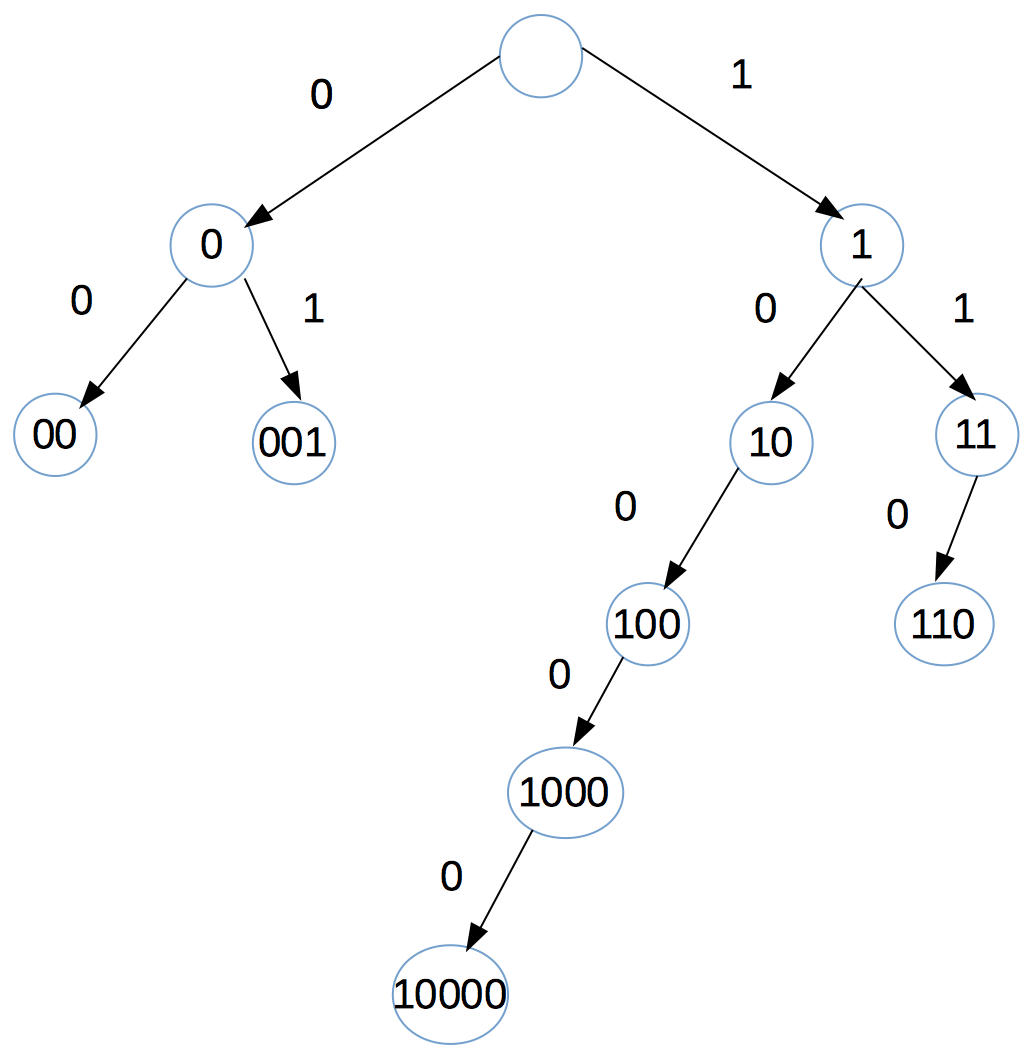
\includegraphics[width=12cm]{PHT.eps}
	\caption{Arbre de préfixe}
	\label{PHT}
	\end{figure}	

\newpage	
	
\section{F-PHT}
	Un fragment est un morceau de bits. On considère un filtre de Bloom de taille \textit{m}. Le système découpe ce filtre en \textit{f} fragments de taille identique. Par convention, ces fragments sont numérotés de \textit{0} à \textit{f-1}, en commençant par le fragment le plus à gauche. L'identifiant de chaque fragment est défini de façon unique.
	
	\begin{table}[!h]
		\centering		
		\begin{tabular}{|l|*{14}{c|}r|}
		\multicolumn{1}{c}{{\scriptsize 15}} &\multicolumn{1}{c}{}&\multicolumn{1}{c}{}&\multicolumn{1}{c}{}&
		\multicolumn{1}{c}{}&\multicolumn{1}{c}{}&\multicolumn{1}{c}{}&\multicolumn{1}{c}{}&
		\multicolumn{1}{c}{}&\multicolumn{1}{c}{}&\multicolumn{1}{c}{}&\multicolumn{1}{c}{}&
		\multicolumn{1}{c}{}&\multicolumn{1}{c}{}&\multicolumn{1}{c}{}&\multicolumn{1}{c}{{\scriptsize 0}}\\
		\hline
			1 & 0 & 0 & \multicolumn{1}{c||}{0} & 
			1 & 1 & 0 & \multicolumn{1}{c||}{1} & 
			0 & 0 & 0 & \multicolumn{1}{c||}{0} & 
			1 & 0 & 1 & 0 \\
		\hline
		\end{tabular}
		\caption{Exemple le filtre de Bloom}
		\label{fragment/filtredeBloom}
	\end{table}
	
	Par exemple, un filtre de Bloom de taille \textit{m = 16} bits, il s'est découpé en \textit{f = 4} fragments, donc chaque fragment est de taille $a = \frac{m}{f} = 4$ bits. Le premier fragment est l'ensemble de bits \textit{"1000"} qui se trouve les 4 bits les plus à gauche du filtre. Le dernier est \textit{"1010"}.

	F-PHT est une sorte d'arbre préfixe, au lieu d'utiliser un seul bit, il utilise "multibit", un fragment, qui stocke des filtres de Bloom de taille \textit{m}. Chaque nœud dans l'arbre a la valeur de son fragment de rang \textit{i} comme clé. Comme le PHT, les données sont stockées uniquement dans les feuilles. Pour stocker une donnée, on prend le premier fragment de cette donnée, cherche le chemin étiqueté par cette valeur. Pour chaque rang \textit{i}, on calcule le fragment correspondant au rang \textit{i} et le chemin convenable. A la fin du chemin, la feuille où on doit stocker cette donnée est trouvée.
	
\chapter{Architecture d'un système d'indexation}
\section{Indexation}
	L'indexation consiste à donner accès aux documents à partir d'une indication concernant leur contenu et/ou leur nature (forme, type) \footnote{combot.univ-tln.fr}. La technique utilisée dans ce systèmre est le F-PHT. On construit un arbre logique réparti sur plusieurs machines/serveurs. Tout le monde peut connaître la racine de cet arbre en appliquant une fonction de hachage sur le nom du racine. Le nom de chaque nœud est unique et généré aussi par cette même fonction. 
	
	Plusieurs nœud peut se trouver sur un seul site, chaque nœud maintient ses propres structures de données qui le caractérisent: un identifiant unique \textit{ID} de ce nœud et une table nommée \textit{LocalRoute}.
	\begin{itemize}
		\item Cet \textit{ID} est le chemin unique qui mène au nœud.
		\item La table \textit{LocalRoute} contient soit les données si c'est un nœud feuille soit la route vers ses fils en descendant.
	\end{itemize}
	
	Un nœud se charge de stocker un ensemble de données qui a la même valeur de fragment de rang \textit{i}. Il gère une table \textit{LocaleRoute} qui contient d'un couple de données. Le premier élément est la valeur d'un fragment, le deuxième est l'identifiant de nœud qui gère ce fragment de rang suivant. Ces éléments sont organisés dans la table \textit{LocalRoute<Frag, ID>} de façon suivant:
	\begin{enumerate}
		\item Si c'est une feuille
			\begin{itemize}
				\item L'indice des entrées dans cette table est correspondant avec la valeur de fragment de rang \textit{i+1}. Donc, le premier élément dans le couple stocké est seulement le reste de filtre de Bloom à partir du rang \textit{i+2} jusqu'à la fin. En plus, une seule entrée peut stocker plusieurs couples. Par contre, une entrée peut stocker au plus $\gamma$ éléments. Cette feuille devient un nœud interne en créant des fils de rang \textit{i+1} qui correspondent à chaque entrée dans la table \textit{LocalRoute}. Après le transfert des données vers les fils, cette table sera remplacée par celle d'un nœud, détaillée en dessous.
				\item L'identifiant dans ce cas là est \textit{null}.
			\end{itemize}
		\item Si c'est un nœud, l'indice des entrées est maintenant la valeur de fragment de rang \textit{i+1}, la donnée est l'identifiant de nœud qui se charge de ce fragment.
	\end{enumerate}	
		
	\begin{figure}[!htbp]
	\centering
	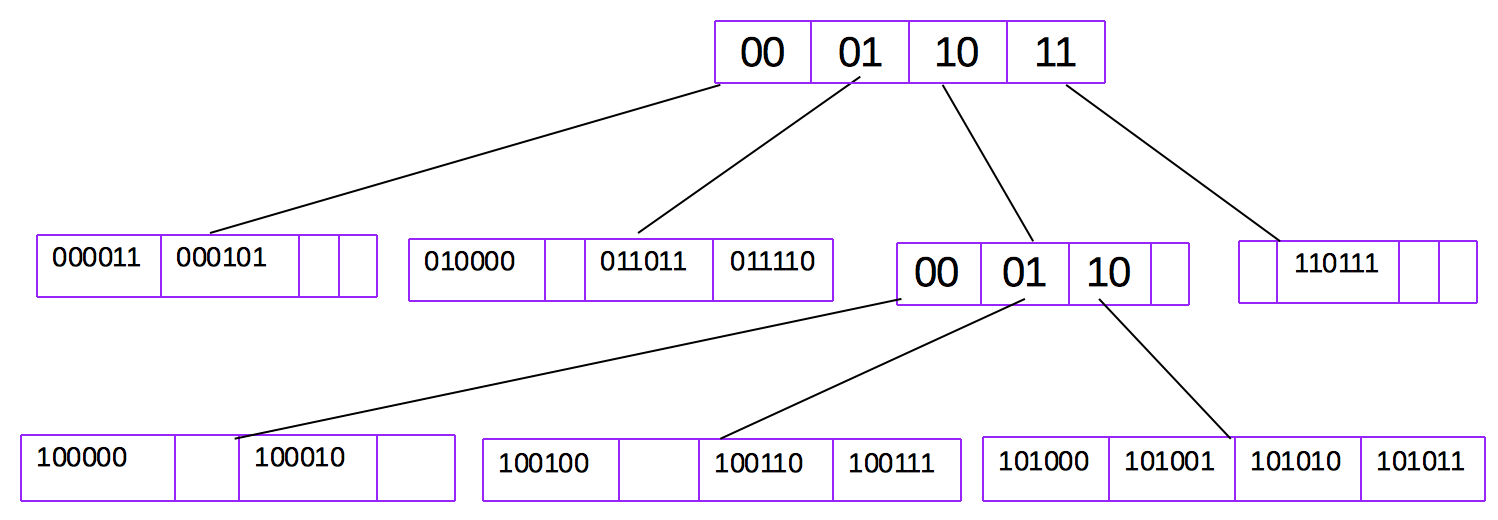
\includegraphics[width=14cm]{F-PHT.eps}
	\caption{Arbre de préfixe}
	\label{F-PHT}
	\end{figure}	

\newpage	

	Dans cette exemple, nous utilisons le filtre de Bloom de taille \textit{m = 8}, il y a 4 fragments de taille \textit{i = 2} bits et $\gamma = 3$. Le nœud \textit{"/10/"} est le résultat après l'éclatement de la feuille \textit{"/10"} car il y a au moins une indice de la table \textit{LocalRoute} contient plus de 3 éléments, par exemple, dans ce cas là, l'indice "00" et "10".

\section{Interface API}
	Ce système offre au utilisateur des fonctions comme :
	\begin{itemize}
		\item créer un nouveau nœud.
		\item supprimer un nœud.
		\item créer un nouveau index.
	\end{itemize}
	
	\begin{figure}[!htbp]
	\centering
	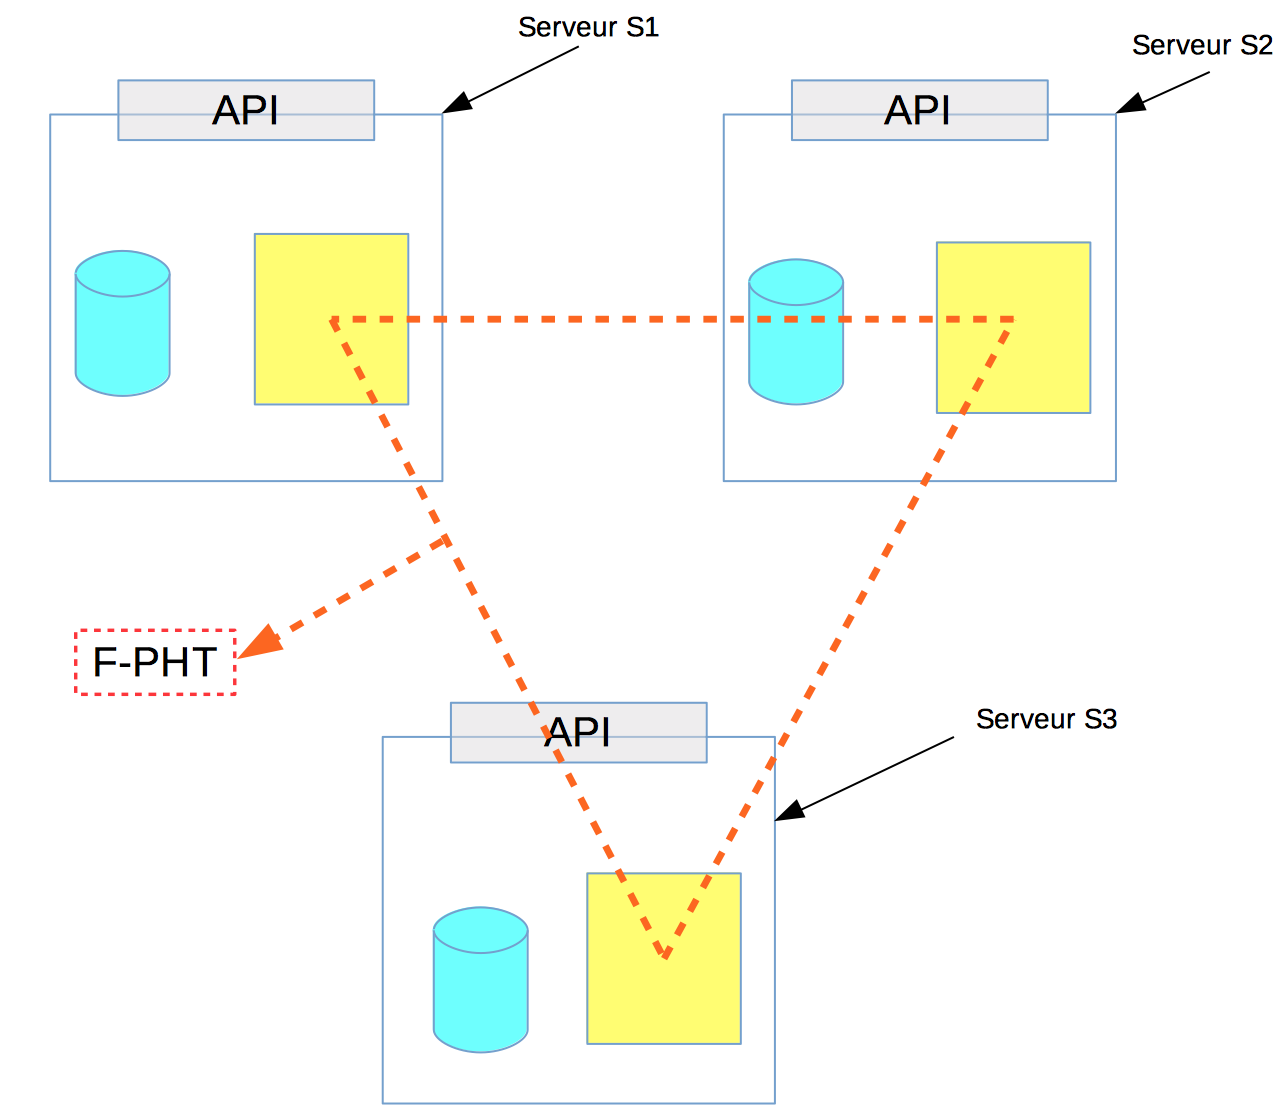
\includegraphics[width=14cm]{systeme-F-PHT.eps}
	\caption{API}
	\label{systeme-F-PHT}
	\end{figure}	
	
	\newpage
	
\chapter{Protocole}
	Ce protocole porte des actions entre le client et le système comme : add, search, remove.
	
\section{Ajout d'un filtre de Bloom}
	Lors que le système reçoit un filtre de Bloom à indexer, il appelle simplement cette méthode \textbf{add}. Cette méthode envoie un message d'ajout à la racine. Ensuite, la racine route ce message jusqu'à la feuille qui s'occupe ce filtre grâce à la valeur de fragment de rang \textit{i}.

\subsection{Cas d'un nœud feuille}
	Lors qu'une feuille reçoit la demande \textbf{add} d'un filtre de Bloom, elle cherche l'indice où le met dans la table \textit{LocalRoute}. Si l'entrée est pleine, pour chaque entrée de la table, elle demande le système de créer un nœud correspondant, et ajoute son identifiant dans la nouvelle table \textit{LocalRoute}. Cette nouvelle table remplace l'autre après les transferts des données vers les fils convenables. Si l'entrée est libre, la feuille ajoute simplement. Elle devient un nœud.
	
\subsection{Cas d'un nœud}
	Un nœud reçoit la demande d'ajout d'un filtre de Bloom est simple, en regardant dans sa table \textit{LocalRoute}, trouve une entrée qui satisfait la requête et la route vers ce fils.
	
\section{Recherche des filtres de Bloom}
	Cette commande \textbf{search} est aussi envoyée vers la racine, par contre, elle renvoie cette requête vers tous les fils qui contient.
	
\subsection{Cas d'un nœud feuille}
	Une feuille reçoit la requête, elle compare la requête avec les filtres dans sa table \textit{LocalRoute}, et collecte tous les filtres qui contiennent la requête. Une fois, tous les filtres satisfaisants sont renvoyés vers la racine.

\subsection{Cas d'un nœud}
	Un nœud compare aussi la requête avec les entrées dans \textit{LocalRoute}, toutes les entrées qui contiennent la requête sont sélectionnées pour récupérer tous les nœuds afin de leur renvoyer la requête.
	
\section{Suppression d'un filtre de Bloom}
	Cette action fonctionne exactement comme l'ajout d'un filtre de Bloom, la racine route la requête de suppression vers le fils qui gère cette requête. Dès qu'elle arrive à la feuille, cette feuille cherche dans sa propre table \textit{LocalRoute} une entrée correspondante et la supprime. Si cette table devient vide après la suppression, elle demande de la supprimer au système, en plus, le système se charge de notifier son père la disparition de son fils pour qu'il puisse supprimer l'entrée de son fils dans sa table de routage \textit{LocalRoute}. Du coup, si sa propre table \textit{LocalRoute} devient vide après la suppression de son fils, il aussi demande de se supprimer au système et notifie son père. Ces opérations continuent jusqu'à quand il n'y a plus de table \textit{LocalRoute} vide.

\end{document}









